%% ----------------------------------------------------------------
%% Currentwork.tex
%% ---------------------------------------------------------------- 
\chapter{Effect of Energy Storage Capacity on Power-Neutral Computing} \label{Chapter:Work2}

% Old: This chapter presents a preliminary work on evaluating the effect of energy storage size on forward progress when given an increased capacity (compared to PN systems) of the energy storage under a control scheme adopted in prior PN systems. The varying harvested energy is balanced within seconds due to the increased storage capacity, which leads to a more flexible control of performance scaling. 

% Poster Abstract: Energy harvesting sources have inherited temporal and spatial variability, which is previously overcome by large energy buffers in the form of batteries. Power neutral computing is proposed to tackle the problems involved in battery usage, whereby the instantaneous power consumption is matched with the instantaneous harvested power through dynamic performance scaling with a minimum storage. However, a PN system has to scale its performance and power consumption quickly and passively, rather than actively select the operating points, which might not be ideal in terms of forward progress. This poster evaluates the forward progress when given an increased capacity of the energy storage under a control scheme adopted in prior power neutral systems. Simulation results show that the forward progress can be improved by up to 12% when properly designing an energy storage.

Energy-neutral computing is an established paradigm, which balances the harvested energy against the energy consumption over a period of time by incorporating sufficient energy storage. Unfortunately, large energy storage increases the volume and cost of devices. Recently, power-neutral computing has been proposed to exploit harvested power using only negligible energy storage by matching the instantaneous power consumption with the instantaneous harvested power. However, due to over-reduction of energy storage, significant performance variations in power-neutral computing may cause performance loss. This chapter presents how an increased amount of energy storage affects the overall system performance, i.e. application throughput. The optimal amount of energy storage is explored, providing a design consideration for selecting the right amount of energy storage in an energy harvesting computing system. As evaluated in simulation based on empirical data of a system-on-chip platform, given a time-varying harvested power trace, properly sizing the energy storage delivers a 14.6\% performance improvement, compared to a state-of-the-art power-neutral system, while maintaining the performance scaling scheme. 

\section{Overview}

% The advent of energy harvesters enables a transformation in the powering method of wireless devices from tethered or battery power into harvested power~\cite{beeby2010energy}. Energy harvesting is to generate electricity from scavenging ambient energy sources, such as light, wind, heat, electromagnetic waves, etc. Energy harvesters can significantly prolong the lifetime of wireless sensor nodes~\cite{jayakumar2016energy}. However, energy harvesting sources have inherent temporal and spatial variability, which contradicts a basic requirement of conventional electronic devices: a stable power supply~\cite{sudevalayam2011energy}. 

% In order to cope with this challenge, 
EN computing separates the load from the energy harvesting power supply with large energy storage, which smooths out differences between the harvested energy and the consumed energy over a long period, such as a few hours~\cite{kansal2007power}, a few days~\cite{sharma2010cloudy}, one year~\cite{buchli2014dynamic}, etc. EN systems maintain a service level over a required period of time so that the total energy consumption equals the total harvested energy~\cite{kansal2007power}. Large energy buffers in EN computing work well in compensating and balancing energy variation, which ensures task execution whether the harvested power is available or not. However, the widespread use of batteries and supercapacitors poses environmental and maintenance issues~\cite{peng2012throughput, raghunathan2005design}, and increases the volume of devices, which contradicts the design requirements in some cases, e.g. wearable devices~\cite{mitcheson2010energy, acampora2013survey}.

Without adding large energy storage as EN computing does, PN computing efficiently utilizes harvested energy by matching the instantaneous power consumption with the instantaneous harvested power. However, strict power tracking in PN systems leads to significant performance variations due to the fluctuation of the harvested power. Such variations may reduce the overall performance (the total amount of completed execution divided by execution time) because of a convex relationship between the system power consumption and the clock frequency in DVFS.

Allocating more energy storage than the minimum level can mitigate this performance variation by constraining the variation of the supply voltage, and hence improve the overall performance. However, increasing energy storage also impedes the performance growth after systems are woken up and respond to a power pulse in a limited time. Also, the energy stored in the capacitor below the minimum operating voltage of the system is effectively wasted, and it takes more time to charge up larger capacitors. Therefore, there is a trade-off between the pros and cons of having a certain amount of energy storage with respect to the system overall performance. 

This chapter presents a methodology to improve system performance by selecting an optimal amount of energy storage given time-varying harvested power. The contributions of this work includes
\begin{itemize}
    \item A theoretical analysis of why adding a certain amount of energy storage to the minimum level improves the overall performance in an energy harvesting system adopting DVFS for performance scaling. 
    \item A model of an energy harvesting computing system using experimental data of a SoC platform, and simulations that evaluate the optimal amount of energy storage and explain the system behaviours.
\end{itemize} 

\section{Problem Identification}

Dynamic performance variations are a typical characteristic of PN computing. This section illustrates the reason why reducing the performance variations improves the overall performance in DVFS-based PN computing, and then, why increasing the minimised energy storage in PN computing supports such improvement.

\subsection{Performance Improvement in DVFS}

Theoretically, CPU power dissipation can be expressed as:
\begin{equation} \label{eq:cpupower}
    P_{CPU} = a V + b f + c f V^2
\end{equation}
where $a,b,c$ are constant parameters determined by hardware when the workload is constant, $V$ is the core voltage, and $f$ is the operating frequency of CPU~\cite{travers2015cpu}. When $f$ changes, the minimum voltage requirement for supporting this frequency changes accordingly. Assume that in DVFS settings, $V$ is adjusted to the minimum required level for every $f$, and hence $P_{CPU}$ is reduced to the minimum level. According to Equation~\ref{eq:cpupower}, $P_{CPU}$ is a quadratic function of $f$, and hence this function $P_{CPU}(f)$ is convex, nondecreasing and nonnegative. 
%When the system can execute tasks at different speeds by scaling performance using DVFS, the CPU power consumption is a convex function of the clock frequency (computing speed)~\cite{irani2007algorithms}.

Here, we denote $P(\alpha)$ as the total power consumption of a system when executing applications at speed $\alpha$ (a performance metric according to specific applications, typically linear to the operating frequency). When the system performs a CPU intensive application, $P_{CPU}$ constitutes the majority of $P(\alpha)$ and $P(\alpha)$ is a convex, nondecreasing and nonnegative function of $\alpha$.
%here, 'CPU intensive' is mentioned. But how to make sure that CPU consumption is still a large part when the load is performing other types of workloads, e.g. sensing tasks? Is it rigorous here?

Based on the convexity of $P(\alpha)$, we examine a case when the system is active and uninterruptedly executes tasks over a certain duration, and the performance scaling method of this system is DVFS. The convexity of $P(\alpha)$ leads to a phenomenon that, when consuming the same amount of energy within the same length of time, maintaining a constant speed renders higher overall performance than switching between two speeds. The proof and explanation of this are shown below. 

Assume that there are three points on $P(\alpha)$ at speed $\alpha_1,\alpha_2,\alpha_3$ and $0 < \alpha_1 < \alpha_2 < \alpha_3$, and hence $0 < P(\alpha_1) < P(\alpha_2) < P(\alpha_3)$. When the energy cost of maintaining speed $\alpha_2$ equals the energy cost of switching between $\alpha_1$ and $\alpha_3$ within a time duration $T$, the following equation is met:
\begin{equation} \label{eq:dvfs1}
    P(\alpha_2)T = P(\alpha_1)t + P(\alpha_3)(T-t)
\end{equation}
where $t$ is the time spent in operating at $\alpha_1$. Hence, $t$ can be calculated from Equation~\ref{eq:dvfs1} as:
\begin{equation} \label{eq:dvfs2}
    t = \frac{P(\alpha_3)-P(\alpha_2)}{P(\alpha_3)-P(\alpha_1)} T
\end{equation}
Due to the convexity of $P(\alpha)$, the following expression is met:
\begin{equation} \label{eq:dvfs3}
    \frac{P(\alpha_3)-P(\alpha_2)}{\alpha_3-\alpha_2} > \frac{P(\alpha_3)-P(\alpha_1)}{\alpha_3-\alpha_1}
\end{equation}
and this can be transformed to:
\begin{equation} \label{eq:dvfs4}
    (\alpha_3 - \alpha_1) \frac{P(\alpha_3) - P(\alpha_2)}{P(\alpha_3) - P(\alpha_1)} T - (\alpha_3 - \alpha_2) T > 0
\end{equation}
By substituting Equation~\ref{eq:dvfs3} into Equation~\ref{eq:dvfs4}, we can get:
\begin{equation} \label{eq:dvfs5}
    \alpha_2 T > \alpha_1 t + \alpha_3 (T - t)
\end{equation}

In Equation~\ref{eq:dvfs5}, the left is the computation done by operating at $\alpha_2$ throughout duration $T$ and the right is the computation done by switching between $\alpha_1$ and $\alpha_3$. Equation~\ref{eq:dvfs2} is true, so Equation~\ref{eq:dvfs5} is true. Therefore, operating at $\alpha_2$ outperforms switching between $\alpha_1$ and $\alpha_3$. The improvement on the overall performance $\eta$ in percentage is: 
\begin{equation} \label{eq:dvfs6}
    \eta = \frac{\alpha_2 T - [\alpha_1 t + \alpha_3 (T - t)]}{\alpha_1 t + \alpha_3 (T - t)} \times 100\%
\end{equation}
By substituting Equation~\ref{eq:dvfs3} into Equation~\ref{eq:dvfs6}, this improvement can be expressed as:
\begin{equation} \label{eq:dvfs7}
    \eta = \frac{\alpha_2 [P(\alpha_3) - P(\alpha_1)]}{\alpha_1 [P(\alpha_3) - P(\alpha_2)] + \alpha_3 [P(\alpha_2) - P(\alpha_1)]} \times 100\%
\end{equation}

Based on Equation~\ref{eq:dvfs5} which examines a case of three points, we conclude that oscillating between two frequencies renders less overall performance than maintaining one frequency between them when consuming the same amount of energy in the same time length. We can expand this conclusion to a case of four points, where oscillating between the two outer frequencies delivers lower overall performance than oscillating between two closer frequencies in the middle of them. Likewise, we can further obtain a case applied for several performance points: reducing the varying range of performance in DVFS results in higher overall performance when systems consume the same amount of energy in the same period. Besides, if $\alpha_1$ and $\alpha_3$ in Equation~\ref{eq:dvfs7} represent the highest and lowest computing frequencies of the scaling range, Equation~\ref{eq:dvfs7} represents the upper bound of improvement in the overall performance.

\subsection{Function of Energy Storage}

Based on the aforementioned analysis, this part illustrates how increasing the amount of energy storage above the minimum delivers performance improvement in systems incorporating DVFS.

\begin{figure}[!tb]
    \centering
    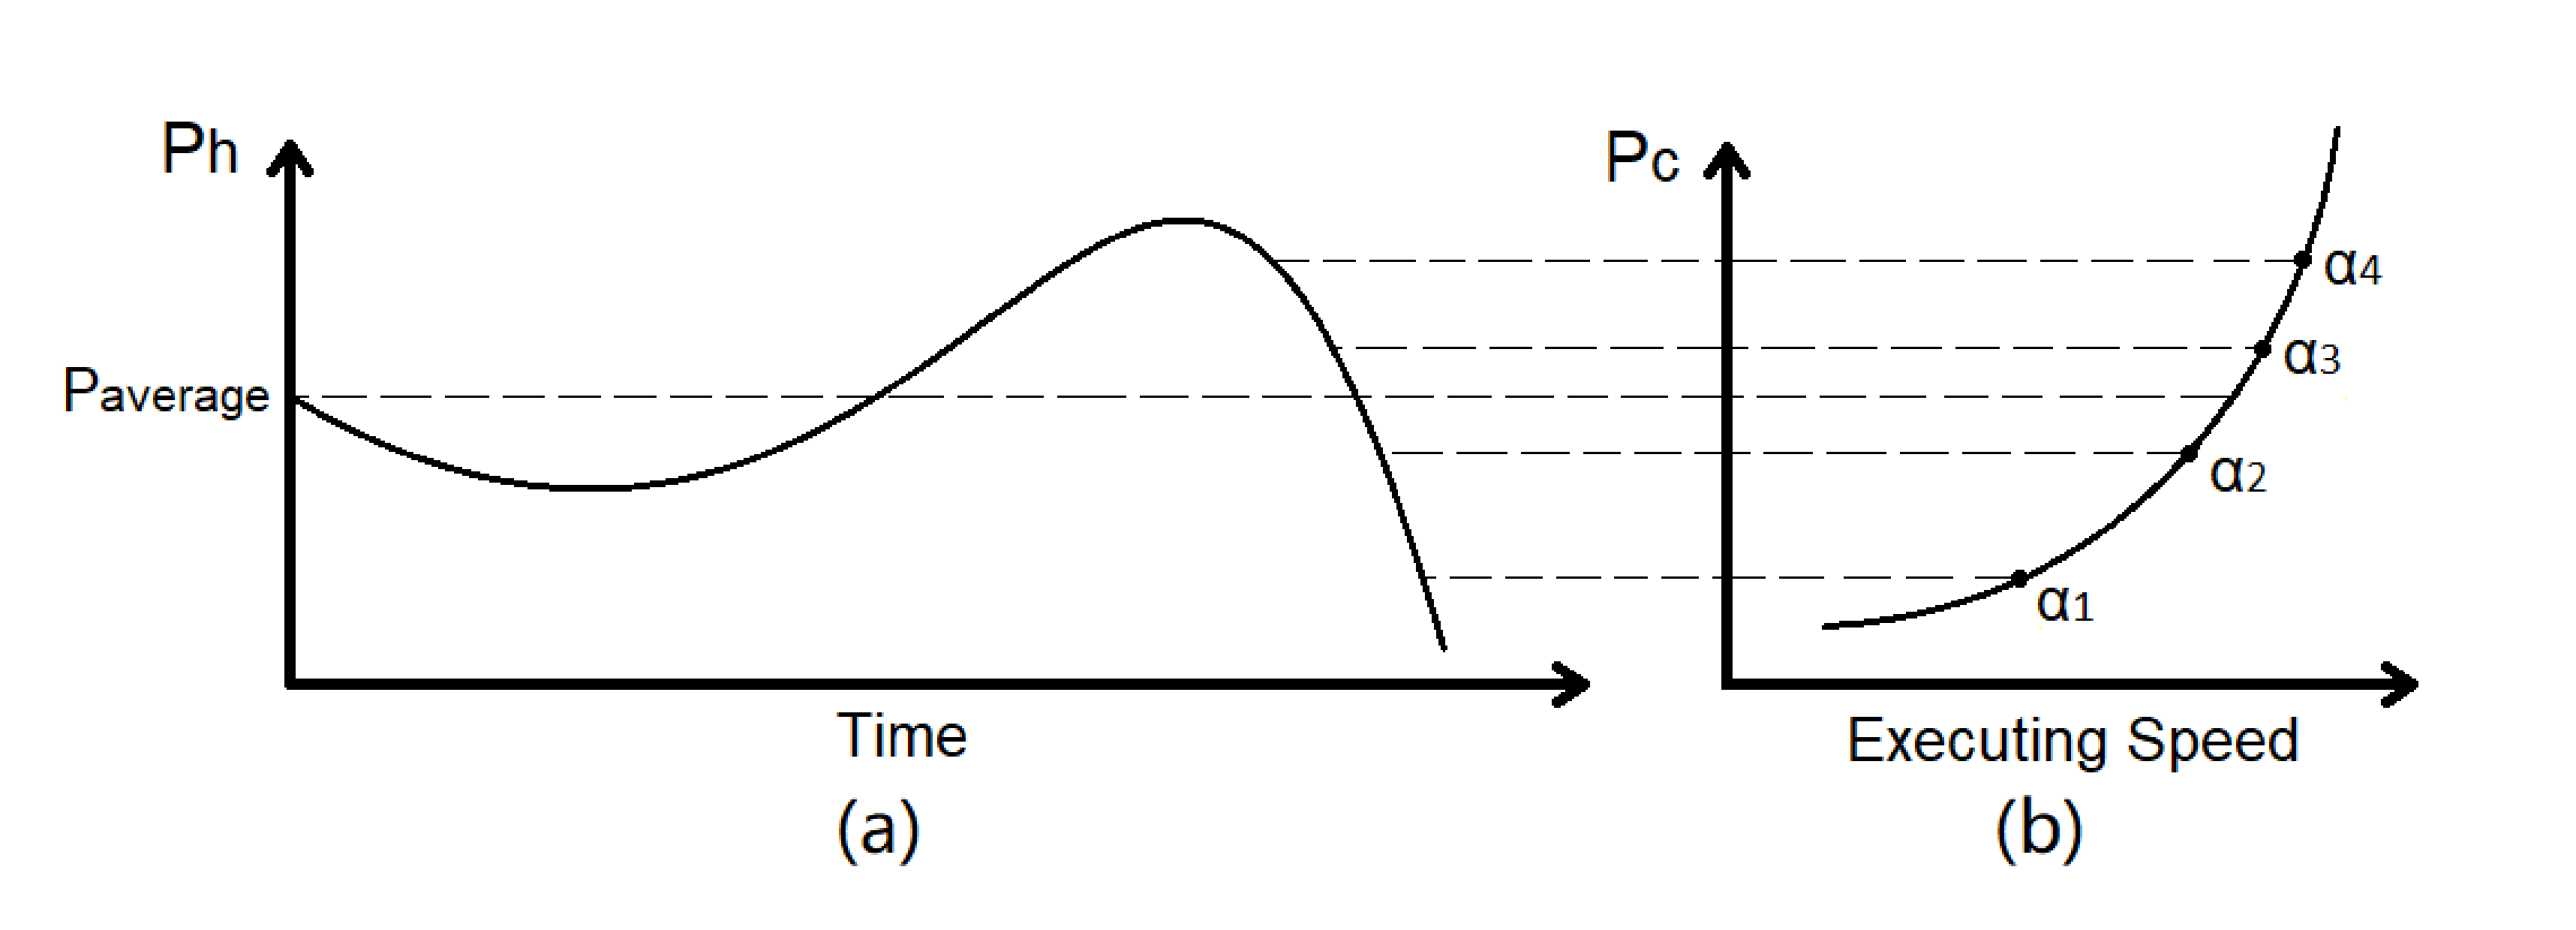
\includegraphics[width=12cm]{figure/work2/pnanalysis}
    \caption{Example of (a) a time-varying harvested power trace and (b) a system's convex power function.}
    \label{Figure:pnanalysis}
\end{figure} 

As illustrated in~\fref{Figure:pnanalysis}, the left is a trace of time-varying harvested power, and the right is a convex power function of a system. $P_{average}$ is the average harvested power during this time duration. $\alpha_2$ and $\alpha_3$ are the closest two operating points to $P_{average}$ on the power function, delivering the best average performance (in practice, the power function is discrete and there is probably not an operating point that exactly consumes $P_{average}$).

In prior PN works~\cite{balsamo2016graceful, fletcher2017power}, when given only minimum storage for the system to switch the operating point, the proposed solution is to match the power consumption with the input power trace as closely as possible, such that the system utilizes the harvested power to the maximum. Specifically, if the small amount of storage can hardly tolerate any power difference, the power consumption can only go just beyond or just below the instantaneous input power anytime. Otherwise, the system stops or the harvested power is wasted. To achieve power matching, the system has to frequently and widely switch among several points between $\alpha_1$ and $\alpha_4$ when responding to the given power trace in~\fref{Figure:pnanalysis}(b).

When the storage is increased from this minimum amount, the system is able to tolerate more temporary power variation. If the storage is large enough to balance the energy over this whole duration, according to the prior analysis, in order to output the highest overall performance within this time duration, the best solution in practice is to oscillate between $\alpha_2$ and $\alpha_3$ for the whole period, rather than scale the frequency across a wider range between $\alpha_1$ and $\alpha_4$. This is why an increased amount of energy storage can improve the overall performance: enabling more energy inequality and allowing more freedom in selecting the operating point and processing tasks. 

However, larger energy storage also introduces longer latency in responding to a power pulse, which leads to inefficient use of harvested energy in both "cold starts" and performance adaptation. Therefore, there is a trade-off between having an amount of energy storage to offset significant power changes and the latency it brings. This trade-off is further evaluated in this work.

\section{System Modelling}

A model is built to evaluate the effect of the amount of energy storage on the overall performance of an energy harvesting computing system. The model structure is based on a simplified architecture of a PN system as shown in~\fref{Figure:modelarch}. This system consists of three main components: an energy harvester, energy storage (a capacitor), and a computing load. These three components are linked by power flows indicated as $P_h$ and $P_c$ representing the harvested power and the system power consumption respectively. Also, the energy harvester is decoupled from the remaining part by a diode to prevent the power backflow, so $P_h \geq 0$ is ensured.

\begin{figure} [!tb]
    \centering
    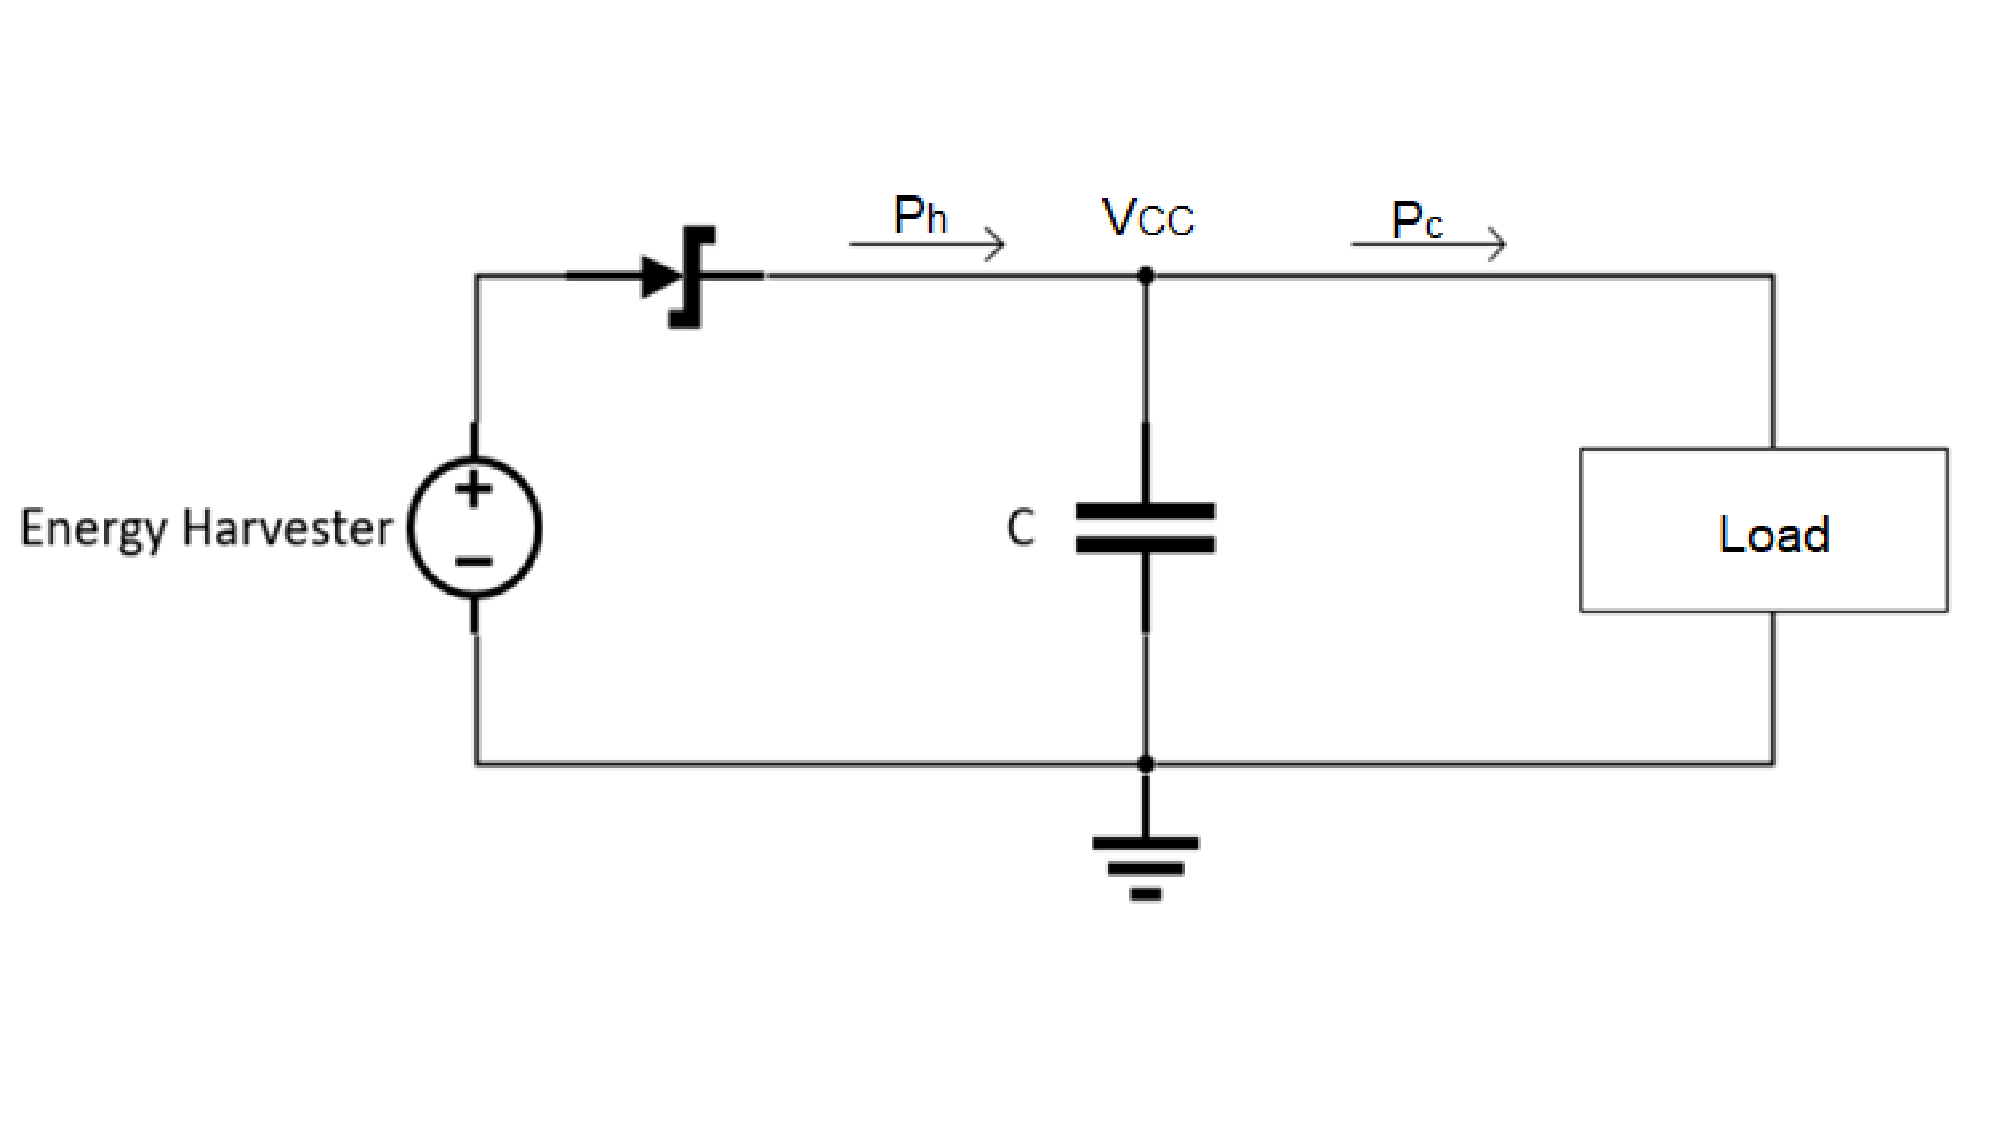
\includegraphics[width=10cm]{figure/work2/modelarch}
    \caption{Simplified architecture of a PN system.}
    \label{Figure:modelarch}
\end{figure} 

\subsection{Energy Harvester}

The energy harvester is modelled by a time-varying power trace, i.e. harvested power against time. This trace can be either taken from the output data of real energy harvesters, or an arbitrary power trace, such that the simulation based on this model can include different power conditions with flexibility. 

\subsection{Energy Storage}

The energy storage is modelled as an ideal capacitor with the following assumptions: a) no leakage; b) 100\% changing and discharging efficiency. The reason for these assumptions is that we aim to focus on how the system exploits the energy storage for balancing the harvested energy and the energy consumption, instead of the power leakage of the capacitor itself. This capacitor model can be expressed as:
\begin{equation}
    E(t) = \frac{1}{2} C V_{cc}(t)^2
\end{equation}
\begin{equation}
    V_{cc}(t) = \sqrt{\frac{2}{C} \int_0^t [P_h(t) - P_c(t)] dt + V_0^2}
\end{equation}
where $t$ is the time; $C$ is the capacitance; $E(t)$, $V_{cc}(t)$ and $V_0$ are the stored energy, the voltage and the initial voltage of the capacitor respectively; $P_h(t)$ and $P_c(t)$ represent the instantaneous harvested and consumed power of the load.

\subsection{Load}

The model of the load is built based on the experimental data of an ODROID-XU4 board. The ODROID-XU4 board is a heterogeneous multiprocessor system-on-chip (SoC) platform based on the Samsung Exynos5422 big.LITTLE SoC with four 'big' high-performance Arm A15 cores and four 'LITTLE' low-power Arm A7 cores. This platform is equipped with hardware support for DVFS which can be utilized with system-level software methods to adjust the operating frequency and the core voltage. Hence, this platform can achieve PN operation and has been used as the experimental platform in prior PN research~\cite{fletcher2017power}.

To obtain the power function of the ODROID-XU4 board, experiments are done by configuring only one A15 core executing threads and one A7 core idle (other cores turned-off), and processing a CPU intensive ray tracing application Smallpt~\cite{beason10}. The operating frequency is scaled from 200MHz to 2000MHz. The performance of this application is measured by the number of rendered frames per second (FPS) at a quality of 4 samples per pixel. The power consumption of the board is recorded by an external power meter. To eliminate the non-deterministic power consumption of the on-board fan as well as to mitigate thermal effects on the CPU power consumption, an external fan is used to control the temperature of the tested board. As shown by the profiling results in~\fref{Figure:pvs11}, this power function presents a convex characteristic, which corresponds to the previous analysis of DVFS, although some parts appear almost linear (e.g. the part between 0.02-0.03 FPS) because the core voltage in these parts is only slightly adjusted according to the DVFS setting of the platform.

\begin{figure} [!tb]
    \centering
    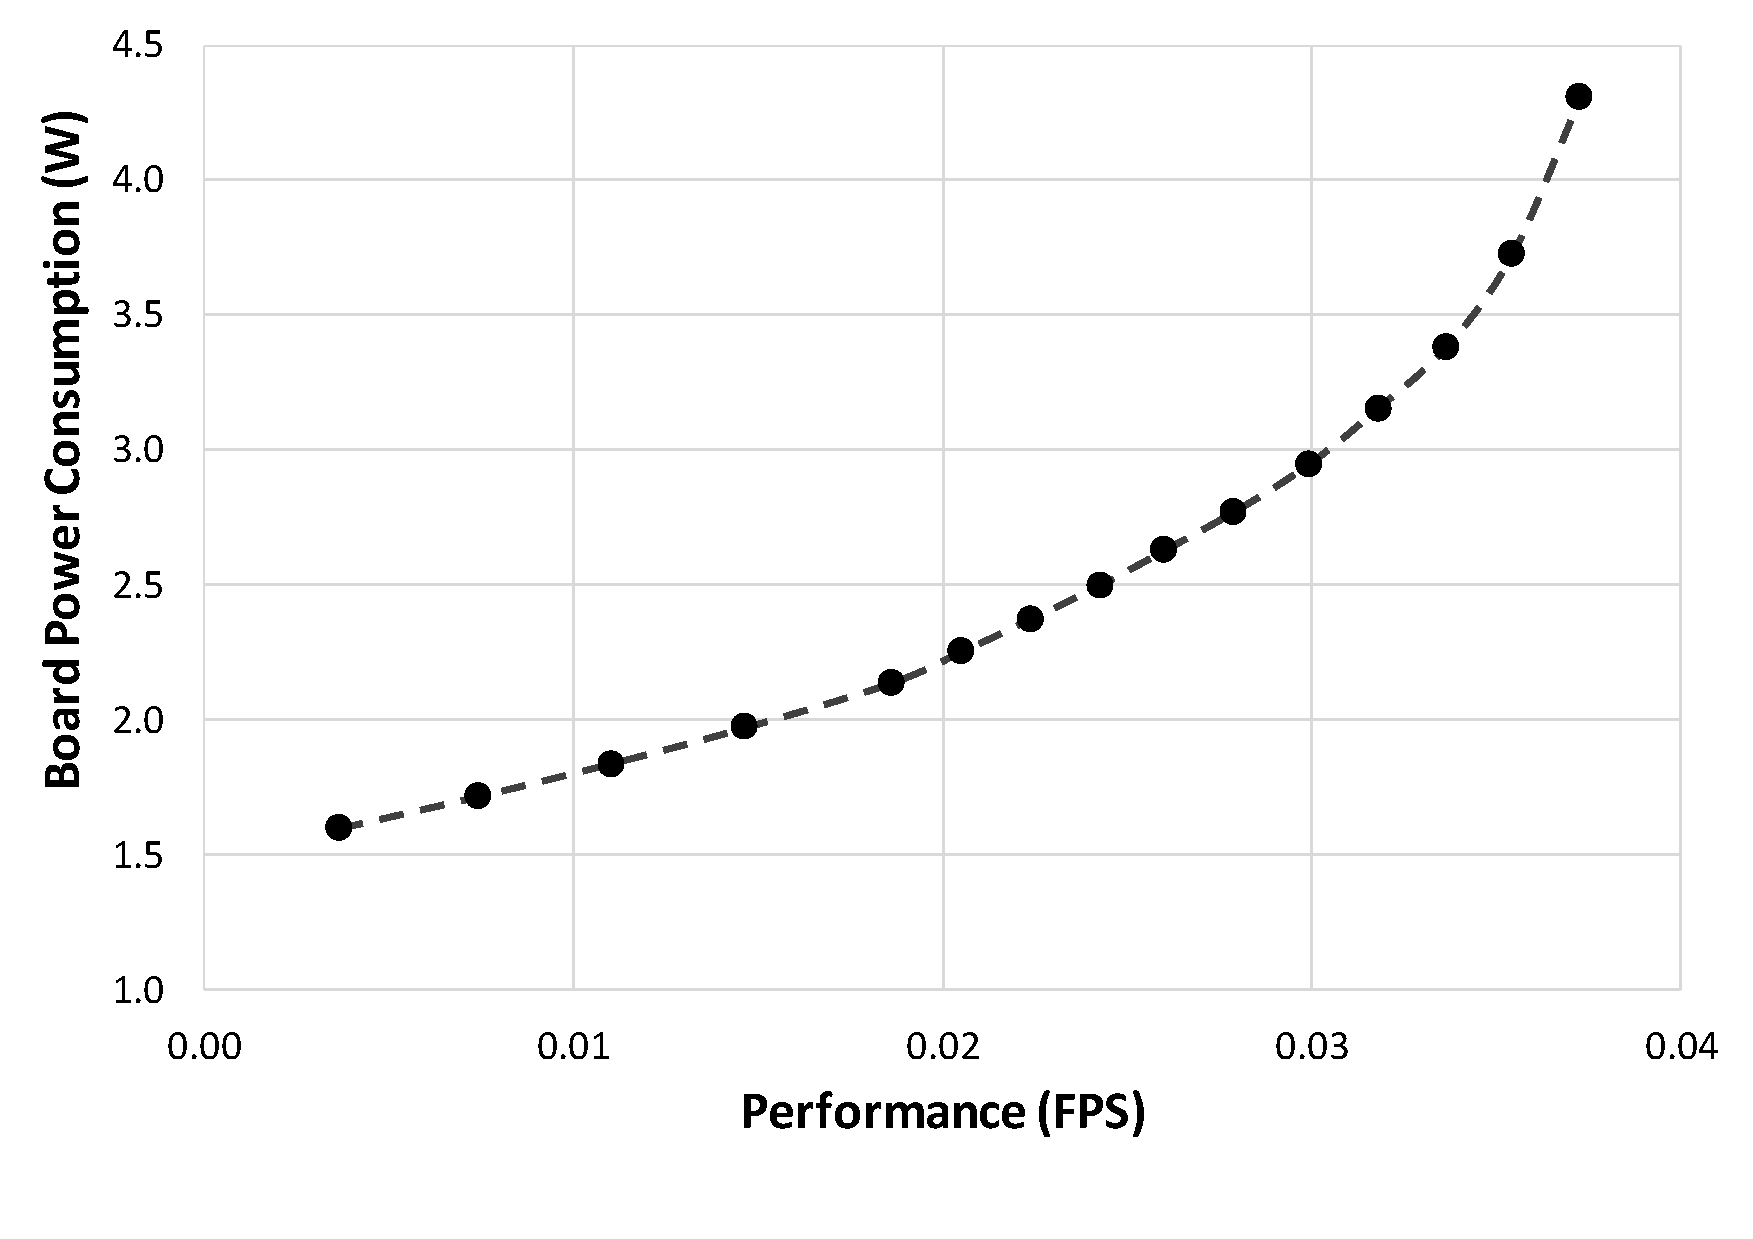
\includegraphics[width=10cm]{figure/work2/pvs11}
    \caption{Profiling results of the ODROID-XU4 board power consumption with one A15 core processing, operating frequency scaled from 200 to 2000 MHz, running a CPU intensive ray tracing application Smallpt at 4 samples per pixel.}
    \label{Figure:pvs11}
\end{figure} 

The load in the model is directly coupled with the capacitor and the changing harvested power causes the variations of $V_{cc}$, while the profiling results are obtained when the system is powered by a stable 5V voltage supply. Consequently, one concern is whether the varying $V_{cc}$ has a considerable impact on the board power consumption. To address this, an experiment is done by switching $V_{cc}$ from 4.1V to 5.7V (the required operating range of supply voltage for the ODROID-XU4 board) under the same core configuration in the profiling test at four frequency levels, which are 200MHz, 1000MHz, 1400MHz and 2000MHz. The results of this experiment in~\fref{Figure:vc_pc} show that the variation of $V_{cc}$ causes up to only 2.1\% difference from the 5V power consumption at each frequency in the total power consumption\footnote{The reason for this is that this board incorporates on-board converters which condition the voltage supply for the SoC from the external power supply, so the board power consumption is not significantly determined by the board supply voltage $V_{cc}$.}. For simplicity, this impact of $V_{cc}$ on power consumption is ignored in our model and following simulation. 

\begin{figure} [!tb]
    \centering
    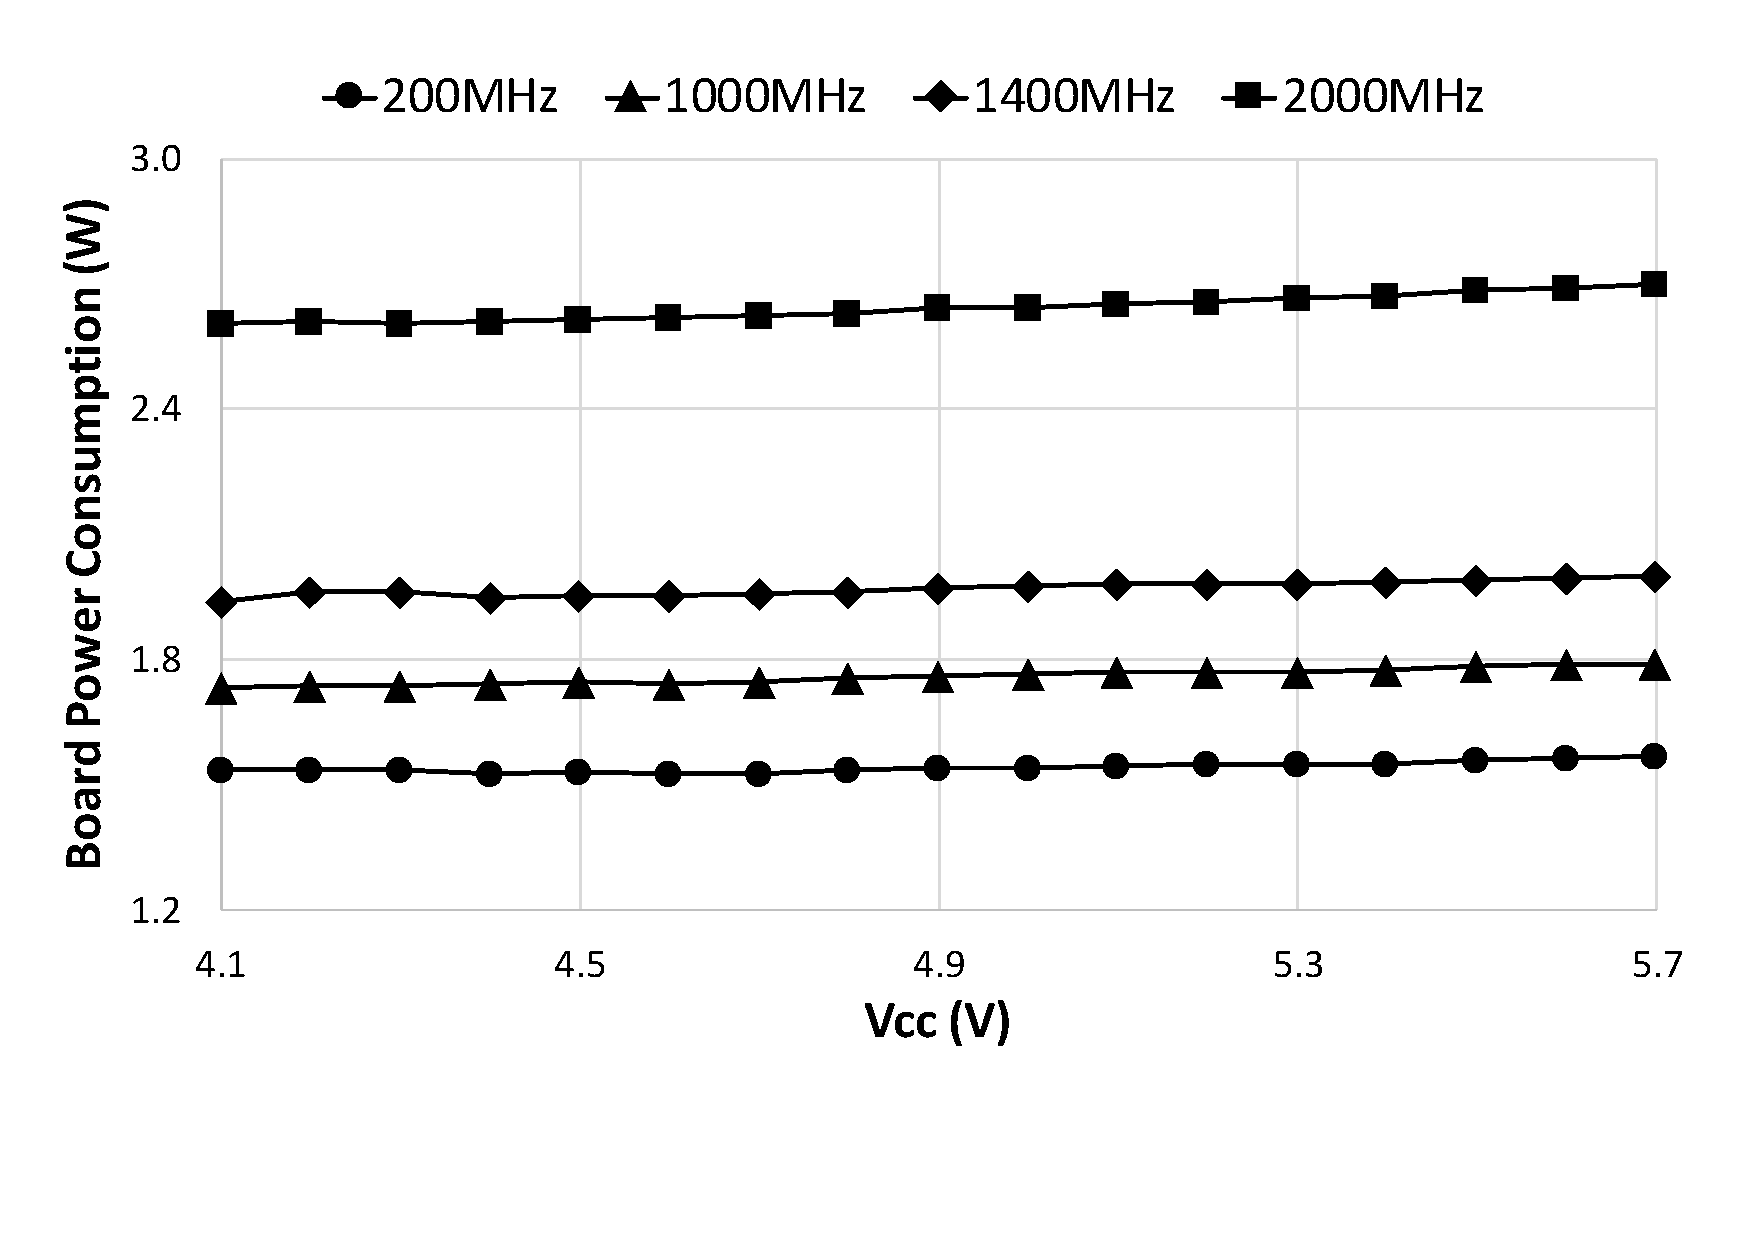
\includegraphics[width=10cm]{figure/work2/vc_pc}
    \caption{Impact of varying Vcc on the board power consumption.}
    \label{Figure:vc_pc}
\end{figure} 

% with a minor difference in frequency settings below 1000MHz, which do not affect the reacting speed
The DVFS control scheme for scaling performance and power of the load in this model is adapted from the state-of-the-art PN work~\cite{fletcher2017power}. The flowchart of the control scheme is shown in~\fref{Figure:pncontrol}. In this control scheme, two dynamic voltage thresholds, $V_{inc}$ and $V_{dec}$, are set for detecting voltage changes in the capacitor caused by power inequality, and then the system scales its performance and power consumption accordingly. The width of these two thresholds is set to the same value (144mV) as in the prior PN work. In practical hardware designs, an external voltage monitor is used to detect voltage changes and generate interrupts for the SoC. When the voltage is detected as crossing a threshold, the frequency is switched to increase or decrease a frequency level and the thresholds are updated accordingly. The time and energy overheads for PN performance scaling is low (0.1\% time overheads and less than 0.8\% energy overheads as reported~\cite{fletcher2017power}), so the frequency switching overheads of time and energy are neglected in our model and simulation.

\begin{figure} [!tb]
    \centering
    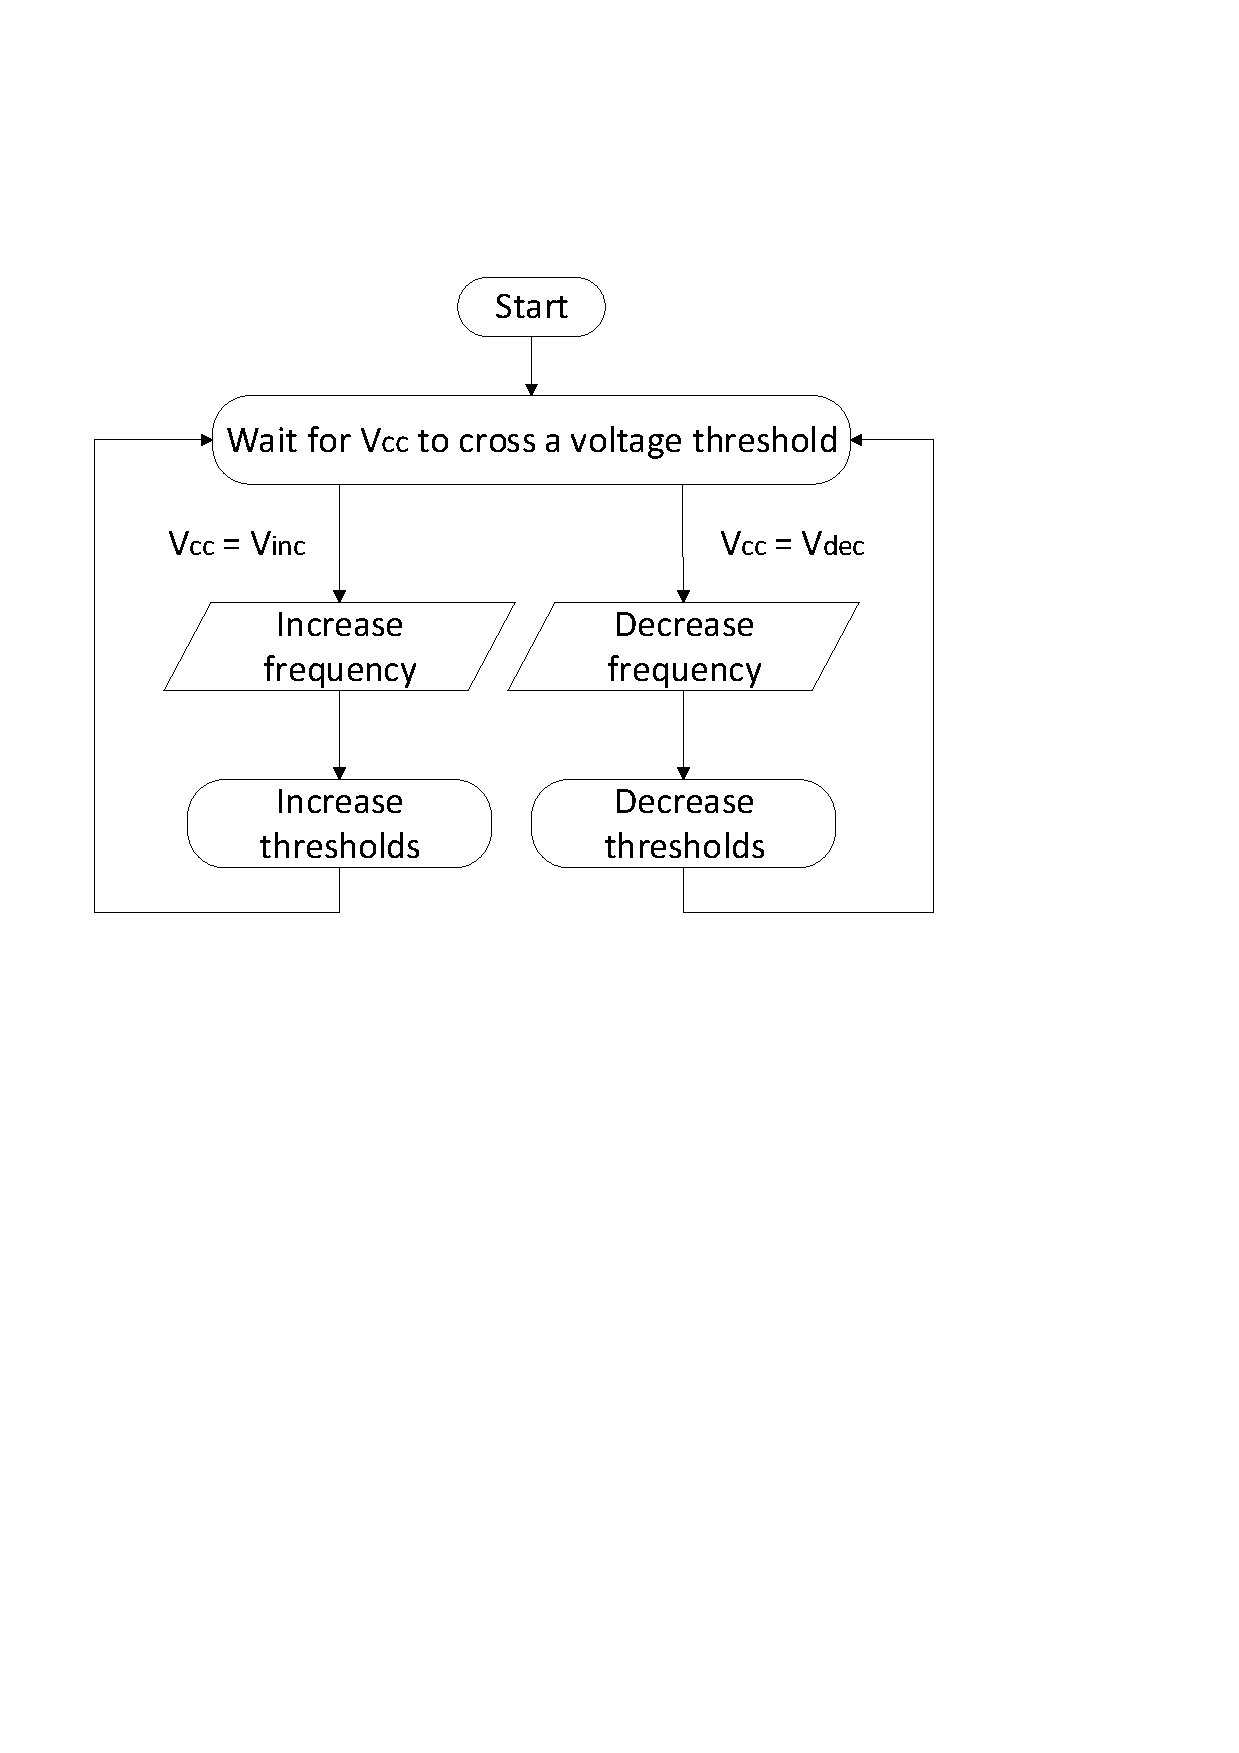
\includegraphics[width=10cm]{figure/work2/pncontrol}
    \caption{Flowchart of the modelled performance scaling scheme adopting DVFS.}
    \label{Figure:pncontrol}
\end{figure} 

\section{Simulations and Results}

The simulation is to evaluate the overall performance when allocated different sizes of energy storage. The range of capacitance is 47mF to 3F with an increase of 1mF per step, which renders a plot with small granularity in capacitance. This range includes a typical case of PN storage (47mF) in a prior PN work~\cite{fletcher2017power} to an amount which can balance almost all the power variation within this duration.

The relationship between the overall performance and the capacitance is presented in~\fref{Figure:frames}. In this test, the PN case (47mF) renders an overall performance of 0.0260 FPS shown at the left of this plot (normalised to 100\%), and this value is used as a comparison for other capacitance cases. When the storage increases, the overall performance increases and reaches a peak at 875mF with an improvement of 14.6\% (0.0298 FPS). This improvement results from narrowing down the varying range of operating frequency, because increasing capacitance reduces the variation of $V_{cc}$ and hence the variation of frequency according to the control scheme. Besides, there are several jump increases in this plot, because the periodicity of the sinusoidal power input causes periodical variation in $V_{cc}$, and hence when such variation is reduced, sometimes a series of performance points are removed.

\begin{figure} [!tb]
    \centering
    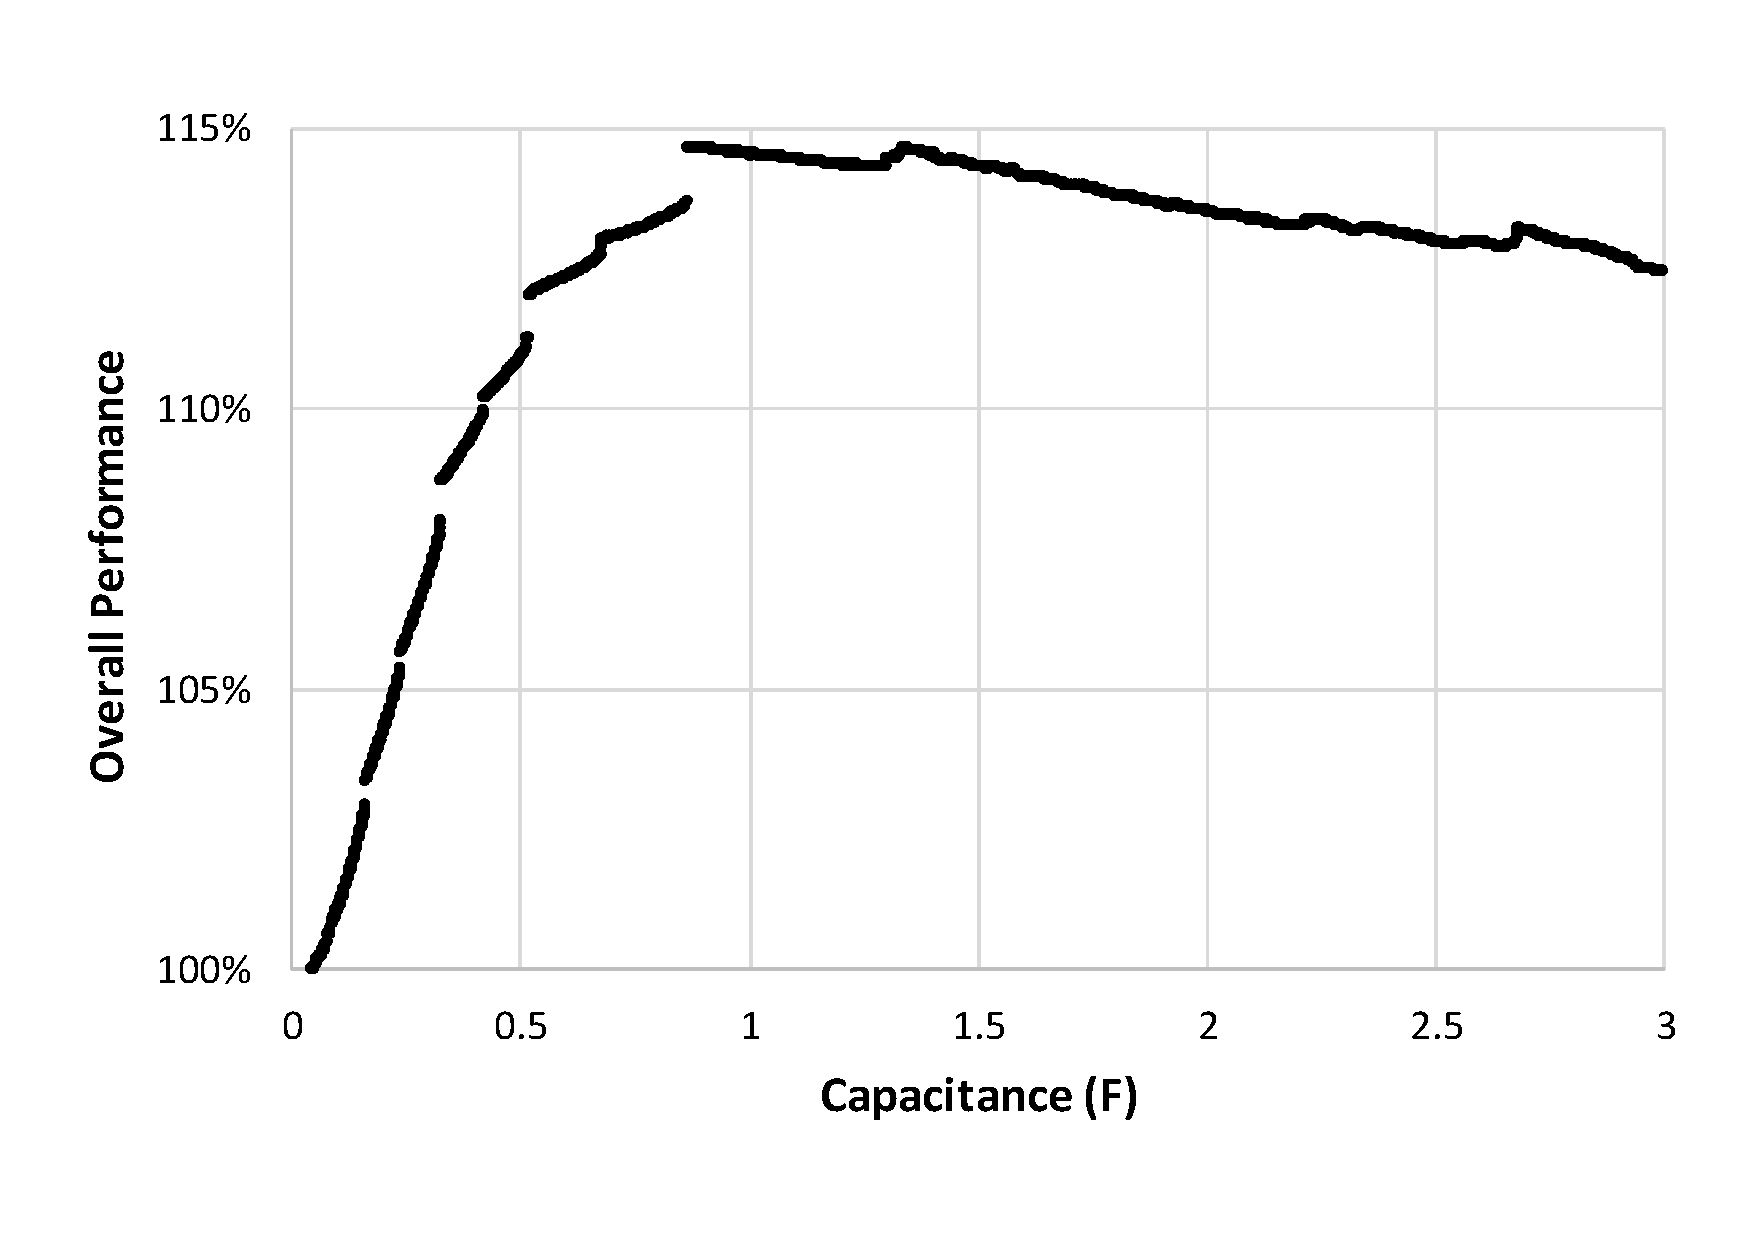
\includegraphics[width=10cm]{figure/work2/frames}
    \caption{Overall performance (calculated by the number of frames/execution time) vs capacitance (0-3F) in the given duration.}
    \label{Figure:frames}
\end{figure} 

However, reducing the variation of $V_{cc}$ by increasing capacitance also slows down the growth of $V_{cc}$ when responding to a power pulse, and hence impedes the growth of operating frequency based on the control scheme. Consequently, with a power pulse available in a limited time, the overall performance decreases if the energy storage is larger than the optimal amount. Therefore, there is a dropping trend of the overall performance when this effect overwhelms the benefit of constraining the range of frequency scaling.

Therefore, there is a trade-off in how much energy storage should be allocated in terms of the overall performance. Properly selecting the size of energy storage according to a specific input power trace can gain an optimal performance improvement (14.6\% in this case).

\begin{figure} [!tb]
    \centering
    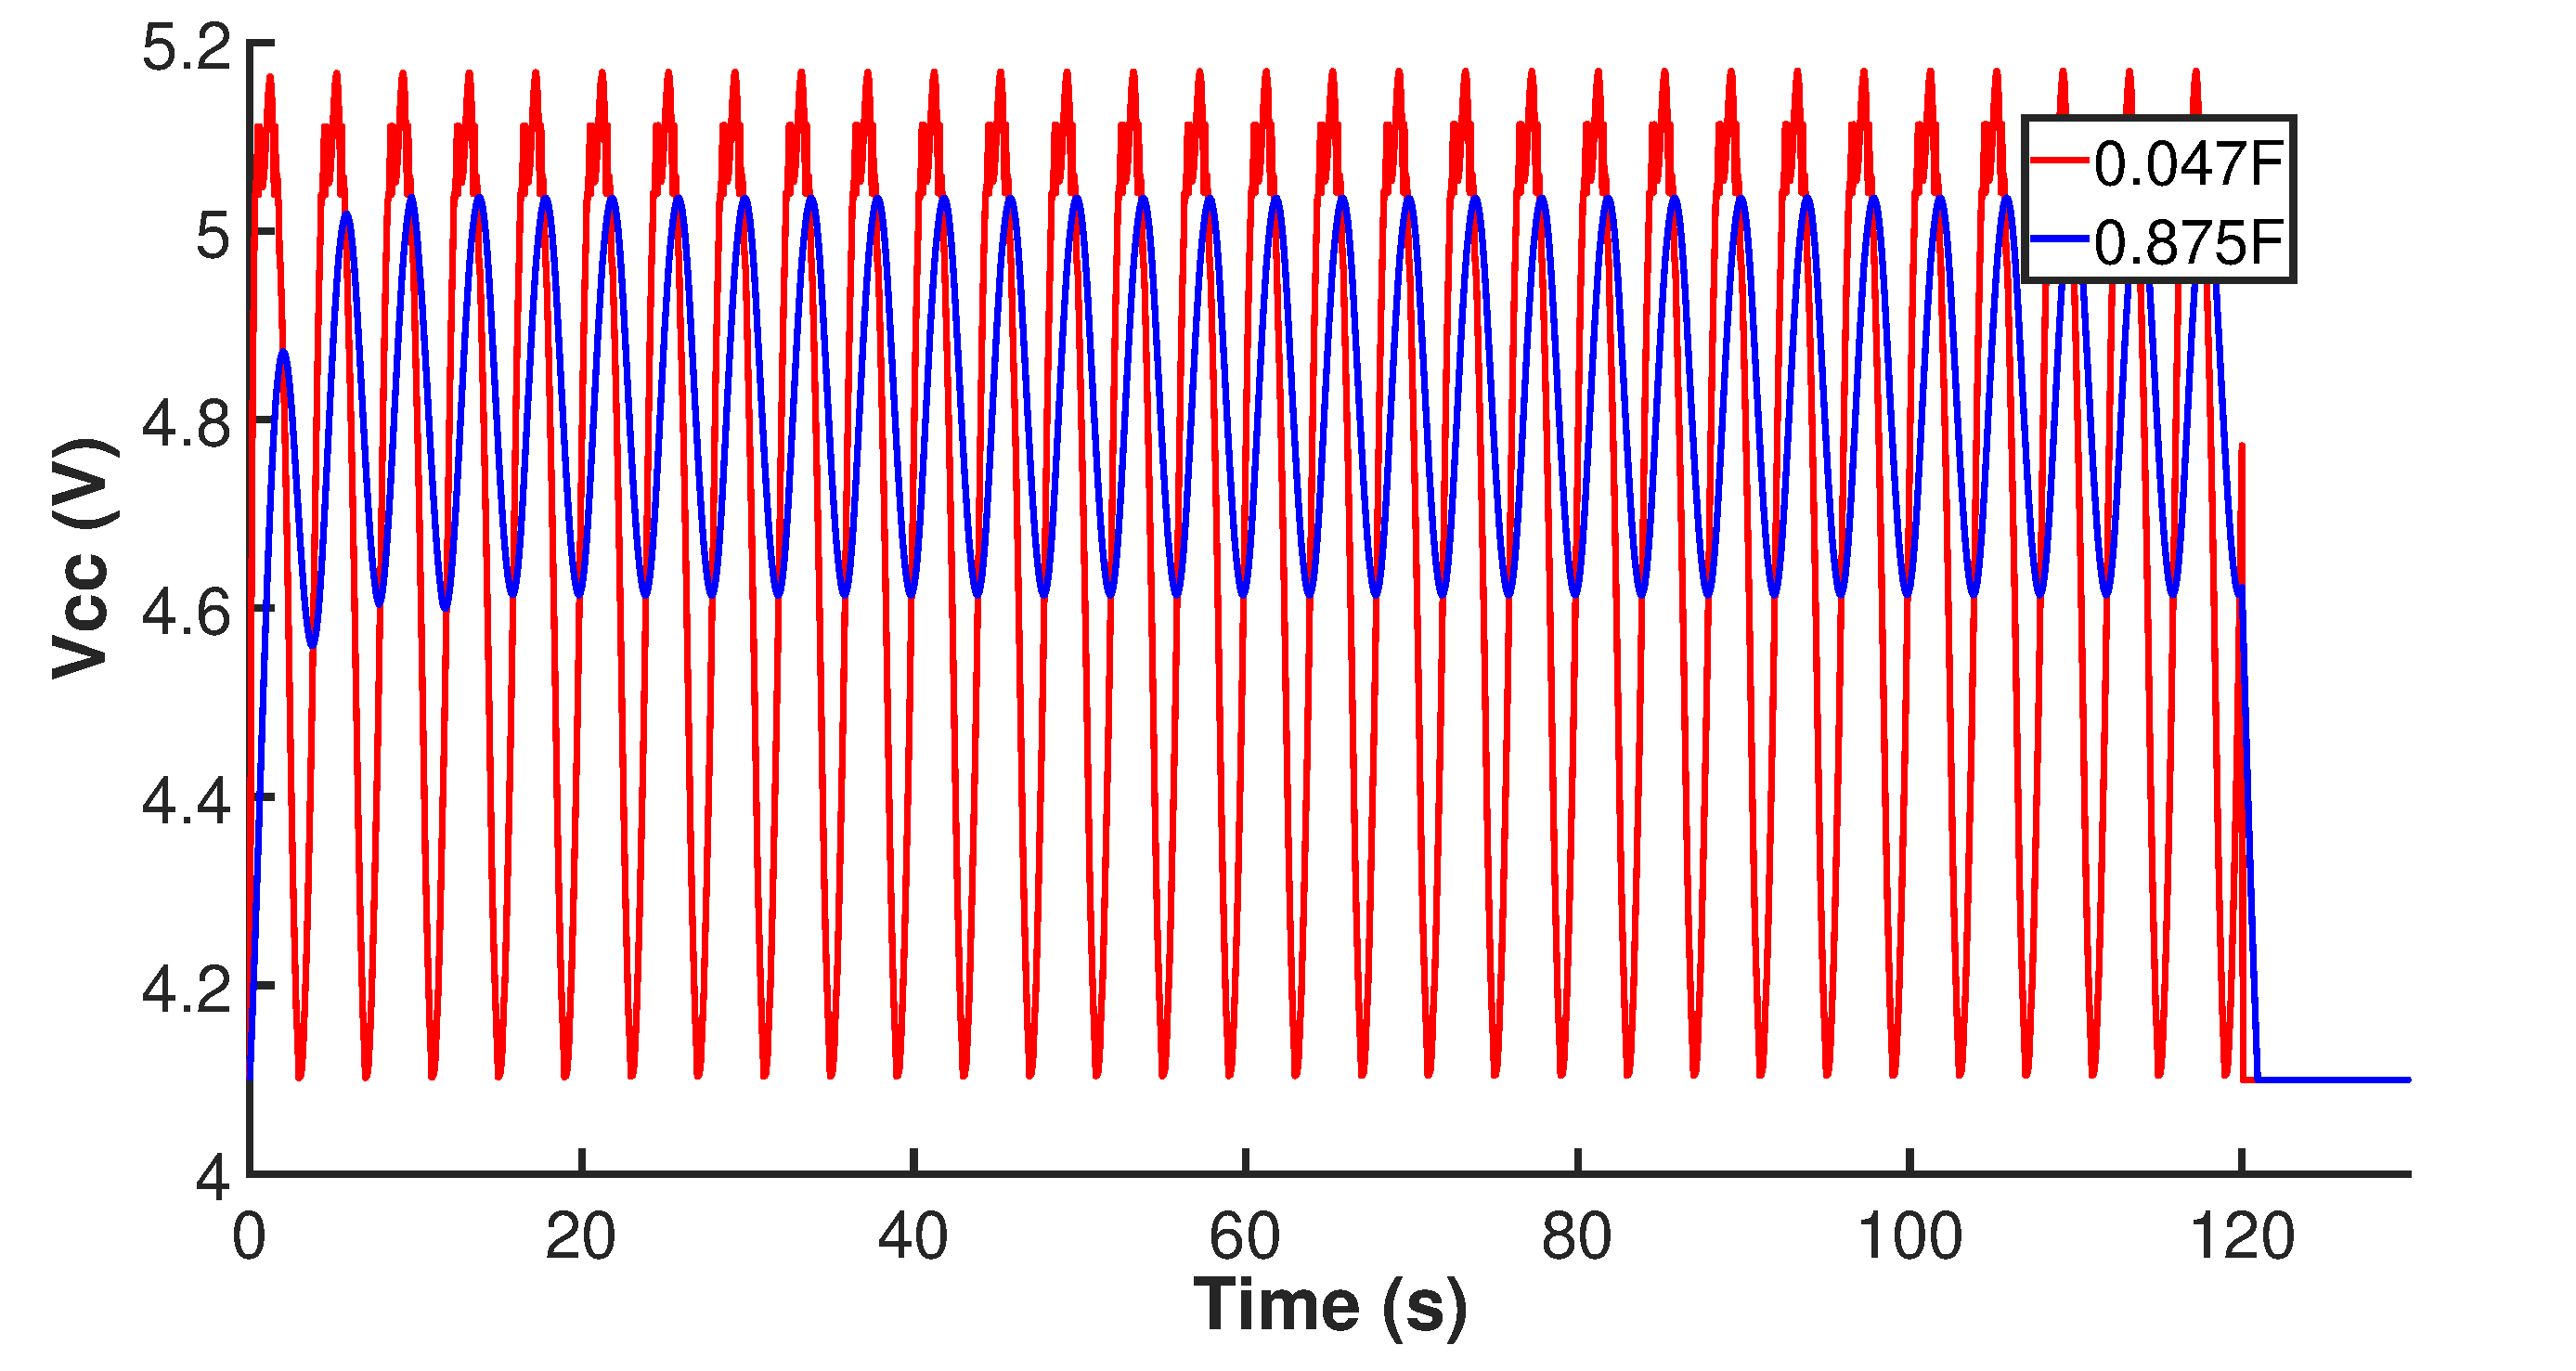
\includegraphics[width=11cm]{figure/work2/vcc}
    \caption{Traces of $V_{cc}$ given 47mF and 875mF energy storage respectively in the given duration.}
    \label{Figure:vcc}
\end{figure} 

\begin{figure} [!tb]
    \centering
    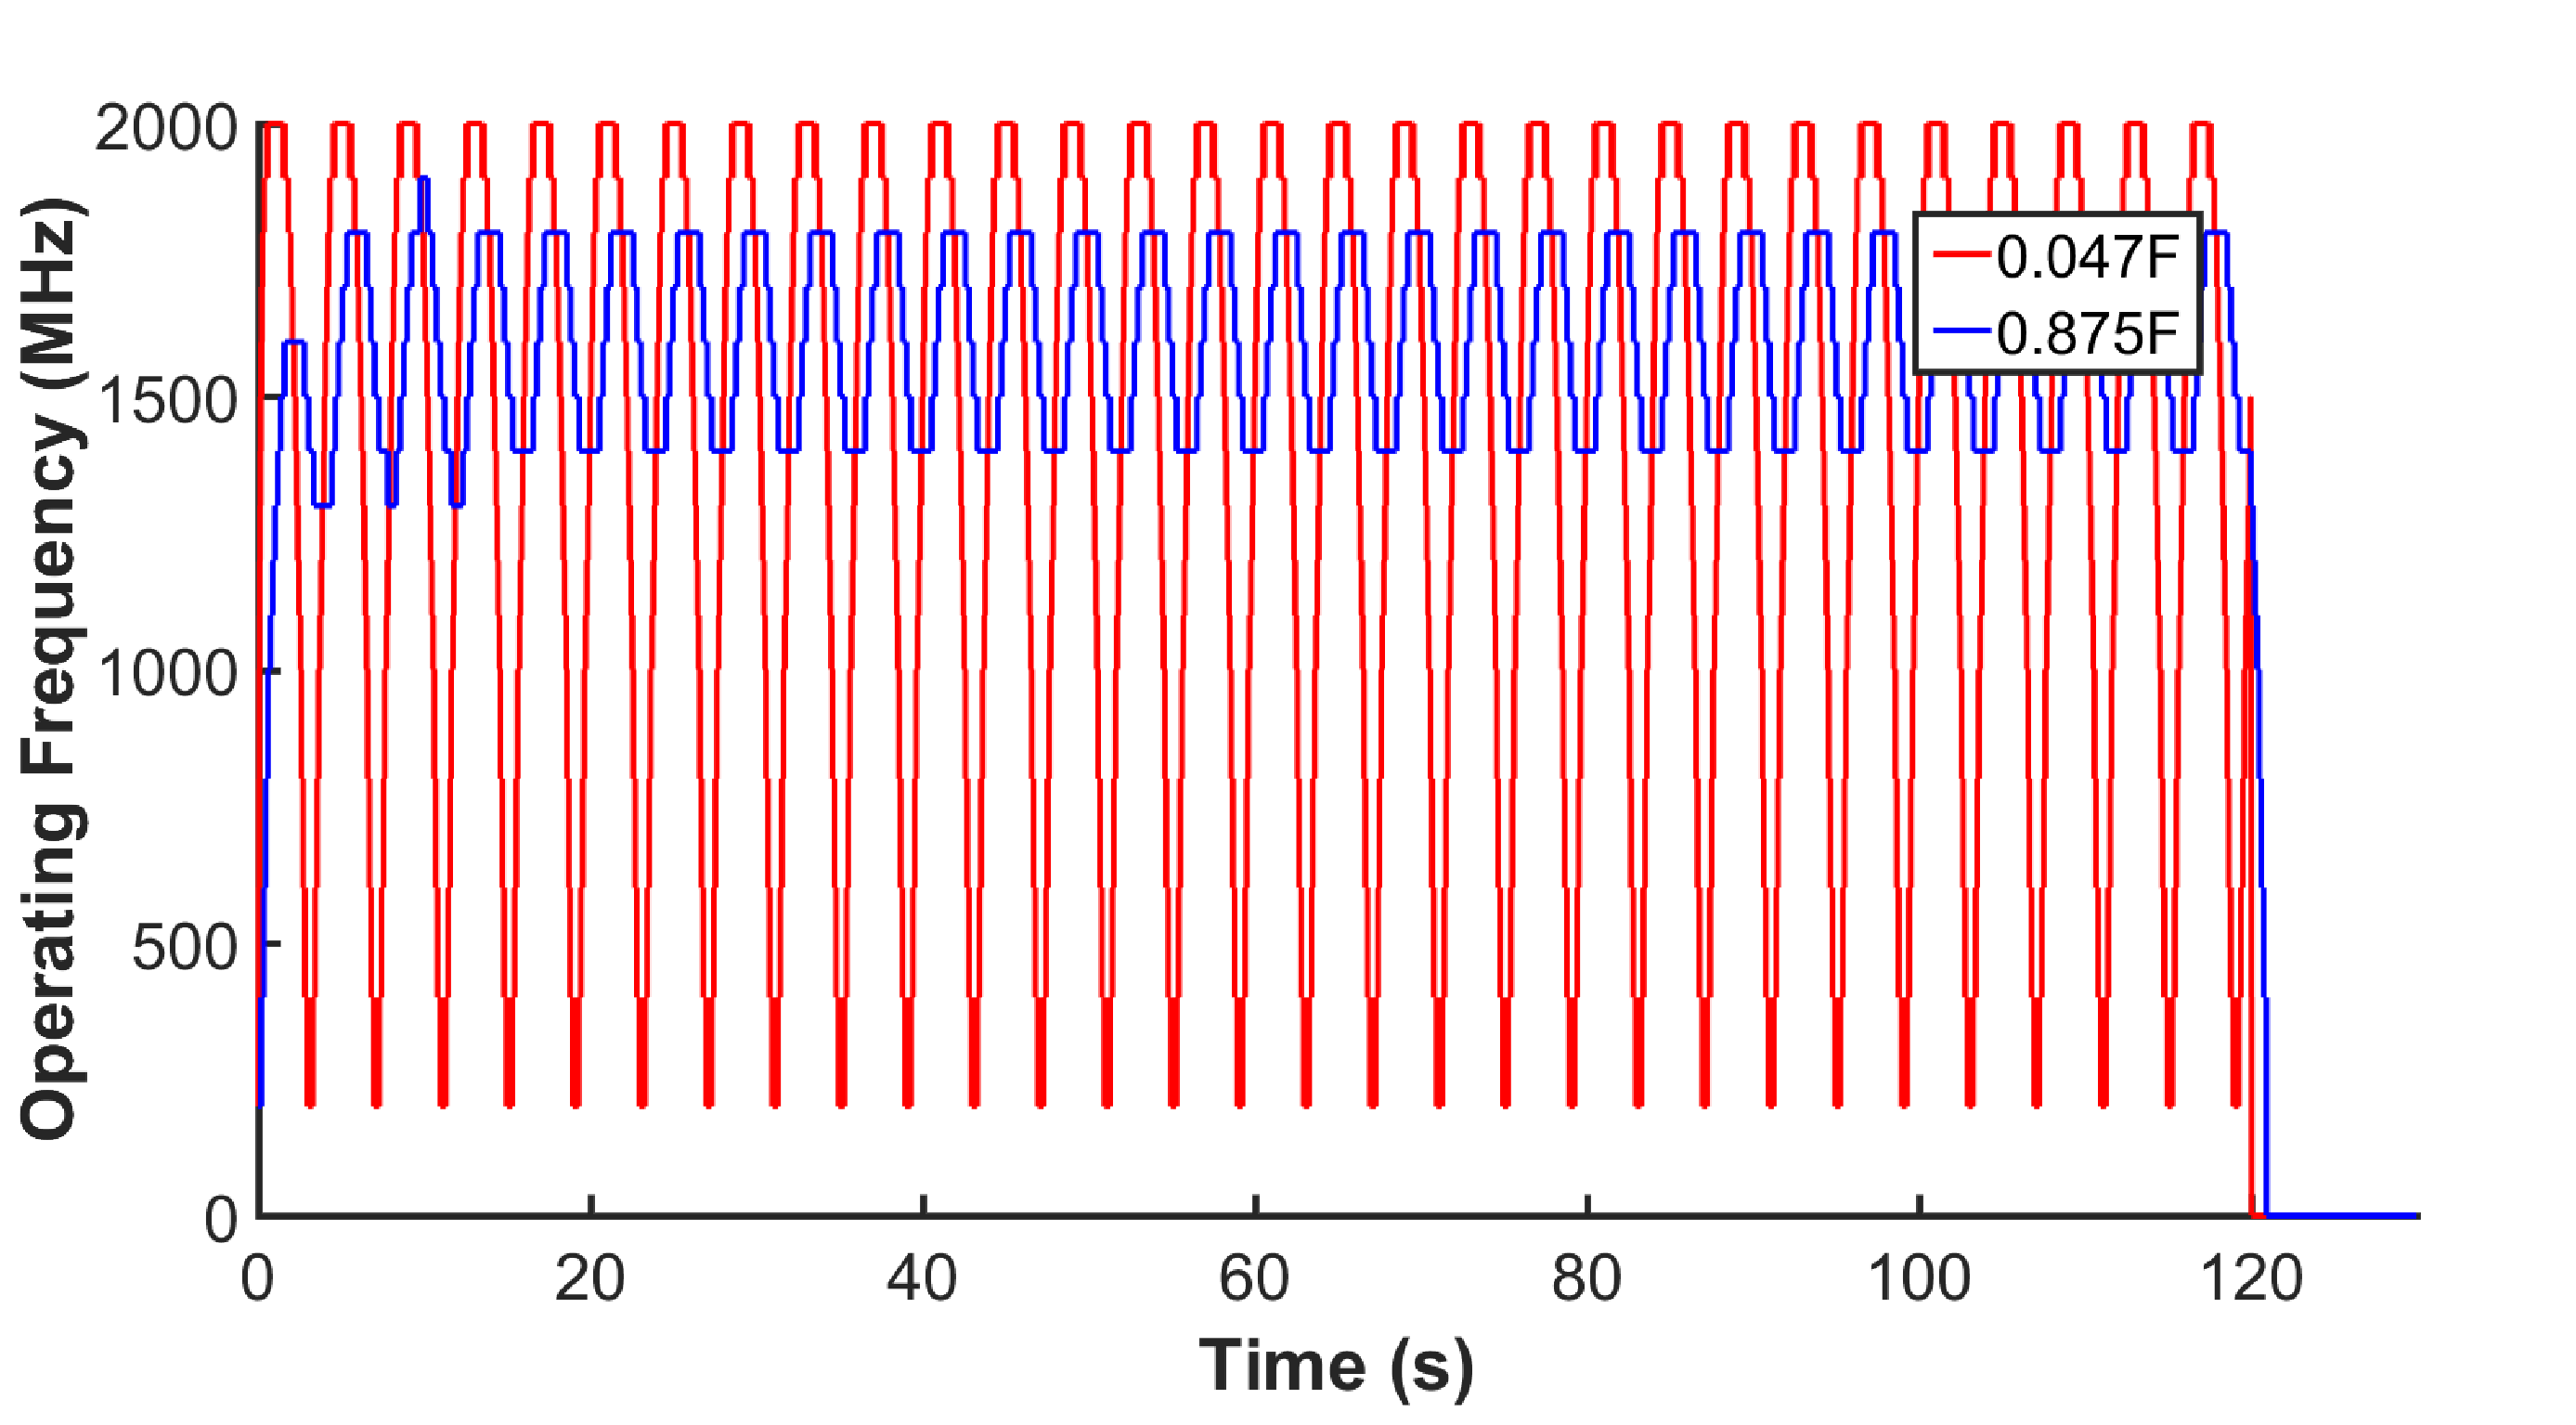
\includegraphics[width=11cm]{figure/work2/op}
    \caption{Traces of operating frequency given 47mF and 875mF energy storage respectively in the given duration.}
    \label{Figure:op}
\end{figure} 

As an illustration of the system behaviour, the traces\footnote{The highest voltage is less than 5.2V, which is below a normal rating voltage 5.5V of supercapacitors~\cite{capacitor}.} of $V_{cc}$ during the test duration given the two typical capacitance values 47mF and 875mF are simulated as shown in~\fref{Figure:vcc}. Comparing the trace of 875mF to the one of 47mF in~\fref{Figure:vcc}, the variation of $V_{cc}$ is reduced due to higher capacitance. Because the control scheme is based on detecting the variation of $V_{cc}$, the operating frequency is controlled within a smaller range. As further results shown in~\fref{Figure:op}, the varying range of operating frequency of 875mF is reduced, which increases the average frequency in this duration and consequently improves the overall application performance. Note that after the input power disappears $V_{cc}$ decreases fast and the execution only lasts for a short time (1.1s for 875mF), so this capacitor is still tiny compared to a typical EN one, focusing on refining performance adaptation rather than balancing long-term energy as EN approaches do.

In addition, with respect to the number of instances of performance scaling, i.e. frequency switching, a simulation result in~\fref{Figure:fsw} shows that this number dramatically drops when the storage increases from the minimum level. For example, this number at 47mF is 978, while the one for 875mF is 256, with a reduction of 73.8\%. The discontinuity in this plot is due to the same reason as the jumps in~\fref{Figure:frames}, namely, the periodicity of the sinusoidal input power. Although time and energy overheads for performance scaling are ignored in our simulation, allocating more storage further curtails the cost of power management in practice, and subsequently allowing more energy and time for program execution.

\begin{figure} [!tb]
    \centering
    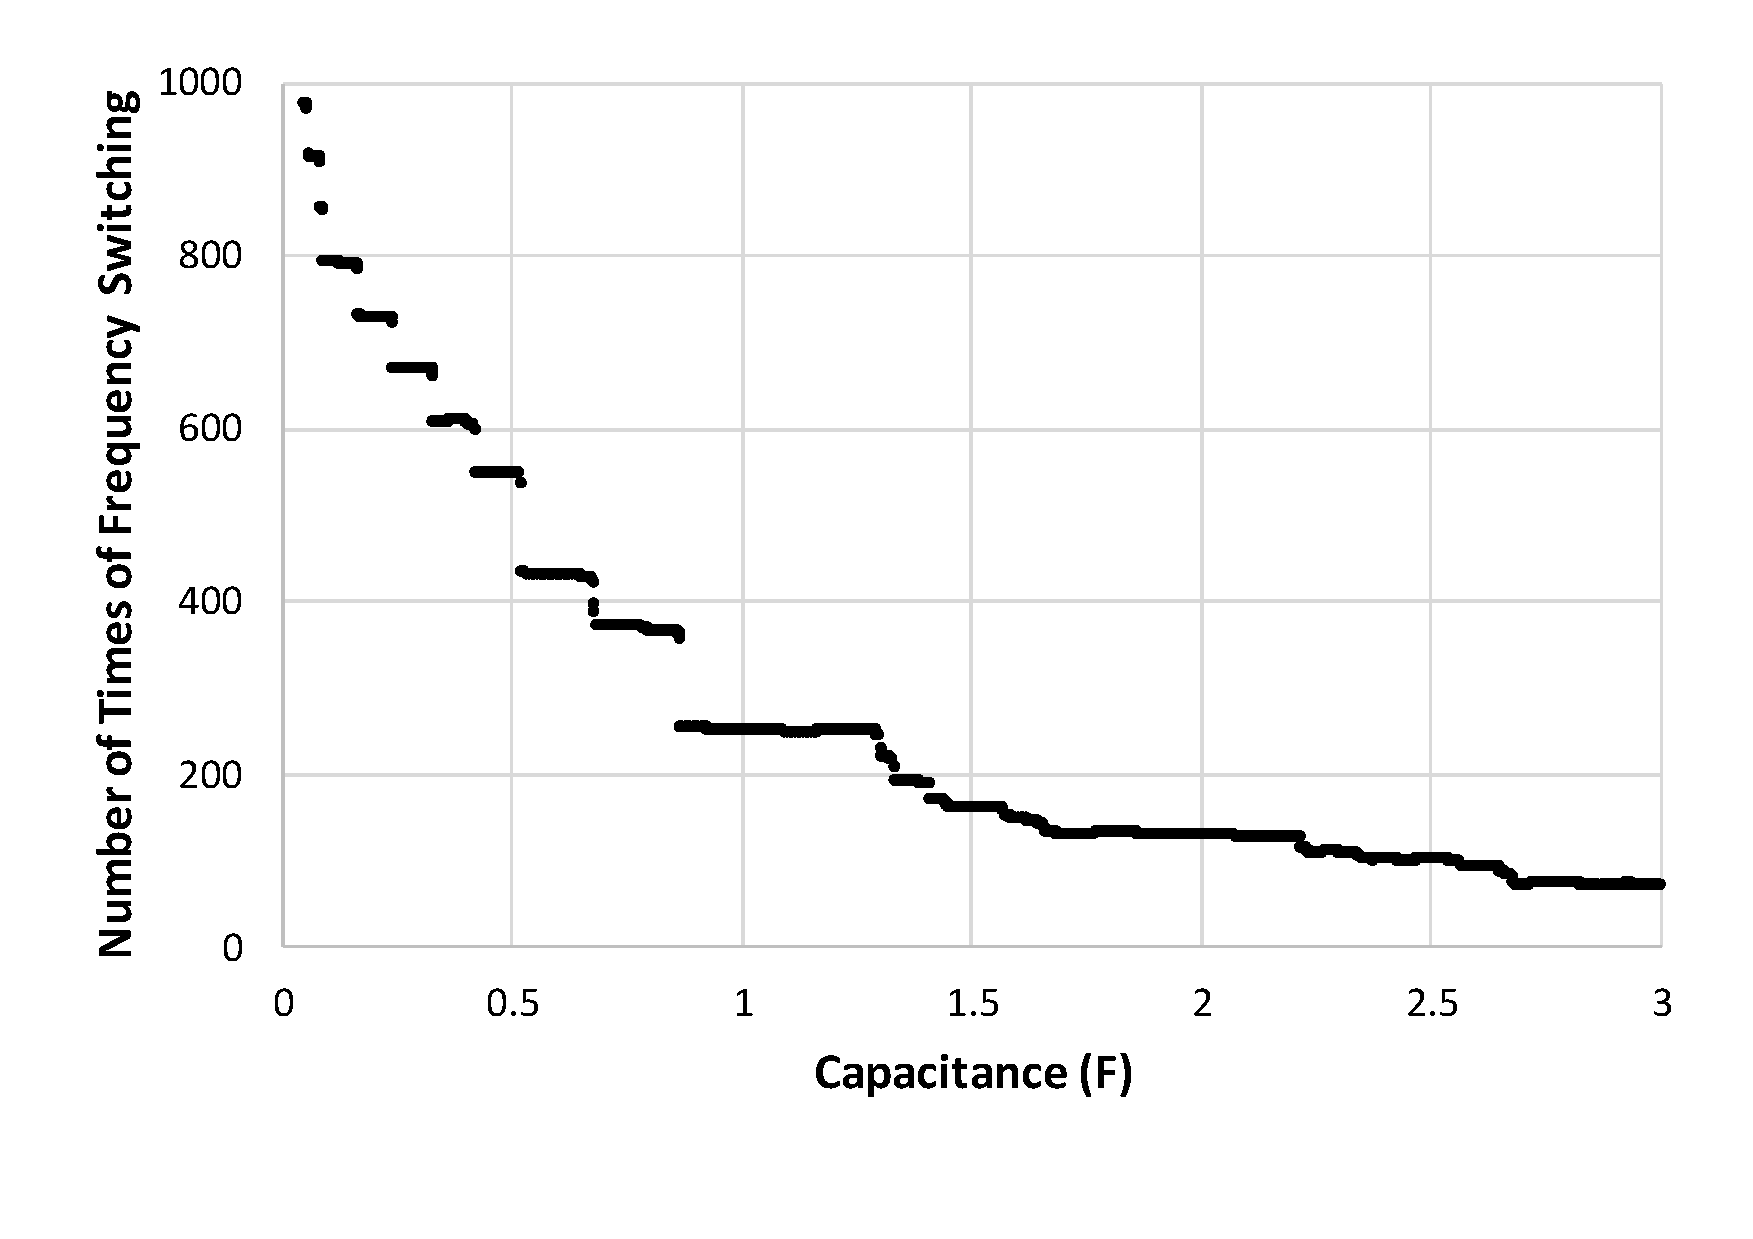
\includegraphics[width=10cm]{figure/work2/fsw}
    \caption{Number of times of frequency switching vs capacitance (0-3F) in the given duration.}
    \label{Figure:fsw}
\end{figure} 

\section{Discussion}
The above simulation indicates that, when properly selecting the capacitor as an energy buffer, it is possible to improve the overall performance in an energy harvesting computing system performing DVFS. However, there are still some concerns.

\textbf{Input Patterns.} It should be mentioned that the input power trace has a significant impact on how much improvement can be achieved. The improvement in computation stems from balancing the power difference in a certain period and then constraining the performance variation. If the input power is rather constant within this period, which implied that there is not much need for scaling performance, this improvement will be insignificant. Hence, the selection of the proper capacitance depends on the particular power trace. 

\textbf{Dimensions of Capacitors.} Also if the volume of the optimal capacitor is too large to meet the design requirements of devices, this approach will be limited by the range of available capacitors. Therefore, it is also necessary to search and conclude how the volume and weight of capacitors changes in manufacture when the capacitance changes. Since we are evaluating the effect of an increased capacity on the forward progress, if the capacitor is too big to suit a device, a trade-off between the performance and device dimensions is introduced.

\textbf{Suspend and Restore.} The analysis and simulations in this report concentrate on the active time of the system, excluding the case of intermittent computing. It is necessary to include a case when the power supply is not sufficient to persistently sustain the system. In such a case, the performance metric for application forward progress should consider the execution rollbacks and record only effective application outputs. 

\section{Summary}

This work analysed the relationship between the amount of energy storage and the overall performance in energy harvesting computing systems when DVFS is incorporated for performance scaling, providing a design consideration for energy storage in energy harvesting sensor nodes. A theoretical analysis illustrated the principle of this relationship. Modelling and simulations were done to evaluate this effect based on experimental data which represented the behaviour of a SoC platform. Simulation results show that there was a trade-off between the pros and cons of reducing the variation of operating frequency. When appropriately designing the energy storage, a 14.6\% speedup in application execution can be gained given a time-varying sinusoidal power trace in our simulation case. 

Further experimental evaluation should be addressed by tests with different types of real energy harvesters, and how to define a proper size of energy storage according to different power characteristics of various energy sources is still a question. Moreover, research attention can be paid to considering how to design a refined power management scheme with a certain amount of energy storage. Finally, the control scheme settings, i.e. the width of the two voltage thresholds and hardware settings for DVFS, determine what the optimal storage size is, and how to adapt the performance scaling scheme in combination with the storage size can be studied in the future. 

% The above analysis and results indicate that properly designing the size of energy storage can improve forward progress in an energy harvesting computing system that adopts DVFS. The three research questions (Section 1.3) have been addressed in a case where sufficient but variable power supply is provided for the system to keep execution.

% Regarding question 1, the theoretical analysis about the convexity of system power function in DVFS reveals how the selection of operating points affects the forward progress, and this is validated by simulation results where a reduction in switching of system clock frequency leads to more forward progress. 

% Regarding question 2, this report provides an explanation for why the minimum energy storage used in PN systems constrain forward progress and why increasing energy storage can improve forward progress by enabling more flexible operating point selection. 

% Regarding question 3, the modelling and simulations validate the above analysis by evaluating the optimal storage size for the given control scheme and the given time-varying power input, and inspecting the system behaviours.
% and also why adding too much energy storage reduces forward progress due to longer response latency to power pulses